\figsetstart
\figsetnum{14}
\figsettitle{All Outflows}

\figsetgrpstart
\figsetgrpnum{14.1}
\figsetgrptitle{SMZ 11}
\figsetplot{f14_01.pdf}
\figsetgrpnote{SMZ 11 outflow. The left panel shows the outflow, position angle, nearby sources, and filaments. The velocity range of integration is given by v$_{\rm blue}$/v$_{\rm red}$ in Table~\ref{tab:outflows}and the contours go from $5$ to $50\sigma$ in steps of 5$\sigma$, where $\sigma$ is the RMS error in the integrated map. Symbols are the same as Figure~\ref{fig:stamp}. The right panel shows the mass spectrum with fit, where $\sigma$ is the RMS error in the integrated map. Symbols are the same as Figure~\ref{fig:dmdv}.}
\figsetgrpend

\figsetgrpstart
\figsetgrpnum{14.2}
\figsetgrptitle{SMZ 17}
\figsetplot{f14_02.pdf}
\figsetgrpnote{SMZ 17 outflow. The left panel shows the outflow, position angle, nearby sources, and filaments. The velocity range of integration is given by v$_{\rm blue}$/v$_{\rm red}$ in Table~\ref{tab:outflows}and the contours go from $5$ to $50\sigma$ in steps of 5$\sigma$, where $\sigma$ is the RMS error in the integrated map. Symbols are the same as Figure~\ref{fig:stamp}. The right panel shows the mass spectrum with fit, where $\sigma$ is the RMS error in the integrated map. Symbols are the same as Figure~\ref{fig:dmdv}.}
\figsetgrpend

\figsetgrpstart
\figsetgrpnum{14.3}
\figsetgrptitle{SMZ 21}
\figsetplot{f14_03.pdf}
\figsetgrpnote{SMZ 21 outflow. The left panel shows the outflow, position angle, nearby sources, and filaments. The velocity range of integration is given by v$_{\rm blue}$/v$_{\rm red}$ in Table~\ref{tab:outflows}and the contours go from $5$ to $50\sigma$ in steps of 5$\sigma$, where $\sigma$ is the RMS error in the integrated map. Symbols are the same as Figure~\ref{fig:stamp}. The right panel shows the mass spectrum with fit, where $\sigma$ is the RMS error in the integrated map. Symbols are the same as Figure~\ref{fig:dmdv}.}
\figsetgrpend

\figsetgrpstart
\figsetgrpnum{14.4}
\figsetgrptitle{SMZ 30}
\figsetplot{f14_04.pdf}
\figsetgrpnote{SMZ 30 outflow. The left panel shows the outflow, position angle, nearby sources, and filaments. The velocity range of integration is given by v$_{\rm blue}$/v$_{\rm red}$ in Table~\ref{tab:outflows}and the contours go from $5$ to $50\sigma$ in steps of 5$\sigma$, where $\sigma$ is the RMS error in the integrated map. Symbols are the same as Figure~\ref{fig:stamp}. The right panel shows the mass spectrum with fit, where $\sigma$ is the RMS error in the integrated map. Symbols are the same as Figure~\ref{fig:dmdv}.}
\figsetgrpend

\figsetgrpstart
\figsetgrpnum{14.5}
\figsetgrptitle{SMZ 50}
\figsetplot{f14_05.pdf}
\figsetgrpnote{SMZ 50 outflow. The left panel shows the outflow, position angle, nearby sources, and filaments. The velocity range of integration is given by v$_{\rm blue}$/v$_{\rm red}$ in Table~\ref{tab:outflows}and the contours go from $5$ to $50\sigma$ in steps of 5$\sigma$, where $\sigma$ is the RMS error in the integrated map. Symbols are the same as Figure~\ref{fig:stamp}. The right panel shows the mass spectrum with fit, where $\sigma$ is the RMS error in the integrated map. Symbols are the same as Figure~\ref{fig:dmdv}.}
\figsetgrpend

\figsetgrpstart
\figsetgrpnum{14.6}
\figsetgrptitle{HOPS 10}
\figsetplot{f14_06.pdf}
\figsetgrpnote{HOPS 10 outflow. The left panel shows the outflow, position angle, nearby sources, and filaments. The velocity range of integration is given by v$_{\rm blue}$/v$_{\rm red}$ in Table~\ref{tab:outflows}and the contours go from $5$ to $50\sigma$ in steps of 5$\sigma$, where $\sigma$ is the RMS error in the integrated map. Symbols are the same as Figure~\ref{fig:stamp}. The right panel shows the mass spectrum with fit, where $\sigma$ is the RMS error in the integrated map. Symbols are the same as Figure~\ref{fig:dmdv}.}
\figsetgrpend

\figsetgrpstart
\figsetgrpnum{14.7}
\figsetgrptitle{HOPS 11}
\figsetplot{f14_07.pdf}
\figsetgrpnote{HOPS 11 outflow. The left panel shows the outflow, position angle, nearby sources, and filaments. The velocity range of integration is given by v$_{\rm blue}$/v$_{\rm red}$ in Table~\ref{tab:outflows}and the contours go from $5$ to $50\sigma$ in steps of 5$\sigma$, where $\sigma$ is the RMS error in the integrated map. Symbols are the same as Figure~\ref{fig:stamp}. The right panel shows the mass spectrum with fit, where $\sigma$ is the RMS error in the integrated map. Symbols are the same as Figure~\ref{fig:dmdv}.}
\figsetgrpend

\figsetgrpstart
\figsetgrpnum{14.8}
\figsetgrptitle{HOPS 12}
\figsetplot{f14_08.pdf}
\figsetgrpnote{HOPS 12 outflow. The left panel shows the outflow, position angle, nearby sources, and filaments. The velocity range of integration is given by v$_{\rm blue}$/v$_{\rm red}$ in Table~\ref{tab:outflows}and the contours go from $5$ to $50\sigma$ in steps of 5$\sigma$, where $\sigma$ is the RMS error in the integrated map. Symbols are the same as Figure~\ref{fig:stamp}. The right panel shows the mass spectrum with fit, where $\sigma$ is the RMS error in the integrated map. Symbols are the same as Figure~\ref{fig:dmdv}.}
\figsetgrpend

\figsetgrpstart
\figsetgrpnum{14.9}
\figsetgrptitle{HOPS 44}
\figsetplot{f14_09.pdf}
\figsetgrpnote{HOPS 44 outflow. The left panel shows the outflow, position angle, nearby sources, and filaments. The velocity range of integration is given by v$_{\rm blue}$/v$_{\rm red}$ in Table~\ref{tab:outflows}and the contours go from $5$ to $50\sigma$ in steps of 5$\sigma$, where $\sigma$ is the RMS error in the integrated map. Symbols are the same as Figure~\ref{fig:stamp}. The right panel shows the mass spectrum with fit, where $\sigma$ is the RMS error in the integrated map. Symbols are the same as Figure~\ref{fig:dmdv}.}
\figsetgrpend

\figsetgrpstart
\figsetgrpnum{14.10}
\figsetgrptitle{HOPS 50}
\figsetplot{f14_10.pdf}
\figsetgrpnote{HOPS 50 outflow. The left panel shows the outflow, position angle, nearby sources, and filaments. The velocity range of integration is given by v$_{\rm blue}$/v$_{\rm red}$ in Table~\ref{tab:outflows}and the contours go from $5$ to $50\sigma$ in steps of 5$\sigma$, where $\sigma$ is the RMS error in the integrated map. Symbols are the same as Figure~\ref{fig:stamp}. The right panel shows the mass spectrum with fit, where $\sigma$ is the RMS error in the integrated map. Symbols are the same as Figure~\ref{fig:dmdv}.}
\figsetgrpend

\figsetgrpstart
\figsetgrpnum{14.11}
\figsetgrptitle{HOPS 56}
\figsetplot{f14_11.pdf}
\figsetgrpnote{HOPS 56 outflow. The left panel shows the outflow, position angle, nearby sources, and filaments. The velocity range of integration is given by v$_{\rm blue}$/v$_{\rm red}$ in Table~\ref{tab:outflows}and the contours go from $5$ to $50\sigma$ in steps of 5$\sigma$, where $\sigma$ is the RMS error in the integrated map. Symbols are the same as Figure~\ref{fig:stamp}. The right panel shows the mass spectrum with fit, where $\sigma$ is the RMS error in the integrated map. Symbols are the same as Figure~\ref{fig:dmdv}.}
\figsetgrpend

\figsetgrpstart
\figsetgrpnum{14.12}
\figsetgrptitle{HOPS 58}
\figsetplot{f14_12.pdf}
\figsetgrpnote{HOPS 58 outflow. The left panel shows the outflow, position angle, nearby sources, and filaments. The velocity range of integration is given by v$_{\rm blue}$/v$_{\rm red}$ in Table~\ref{tab:outflows}and the contours go from $5$ to $50\sigma$ in steps of 5$\sigma$, where $\sigma$ is the RMS error in the integrated map. Symbols are the same as Figure~\ref{fig:stamp}. The right panel shows the mass spectrum with fit, where $\sigma$ is the RMS error in the integrated map. Symbols are the same as Figure~\ref{fig:dmdv}.}
\figsetgrpend

\figsetgrpstart
\figsetgrpnum{14.13}
\figsetgrptitle{HOPS 59}
\figsetplot{f14_13.pdf}
\figsetgrpnote{HOPS 59 outflow. The left panel shows the outflow, position angle, nearby sources, and filaments. The velocity range of integration is given by v$_{\rm blue}$/v$_{\rm red}$ in Table~\ref{tab:outflows}and the contours go from $5$ to $50\sigma$ in steps of 5$\sigma$, where $\sigma$ is the RMS error in the integrated map. Symbols are the same as Figure~\ref{fig:stamp}. The right panel shows the mass spectrum with fit, where $\sigma$ is the RMS error in the integrated map. Symbols are the same as Figure~\ref{fig:dmdv}.}
\figsetgrpend

\figsetgrpstart
\figsetgrpnum{14.14}
\figsetgrptitle{HOPS 60}
\figsetplot{f14_14.pdf}
\figsetgrpnote{HOPS 60 outflow. The left panel shows the outflow, position angle, nearby sources, and filaments. The velocity range of integration is given by v$_{\rm blue}$/v$_{\rm red}$ in Table~\ref{tab:outflows}and the contours go from $5$ to $50\sigma$ in steps of 5$\sigma$, where $\sigma$ is the RMS error in the integrated map. Symbols are the same as Figure~\ref{fig:stamp}. The right panel shows the mass spectrum with fit, where $\sigma$ is the RMS error in the integrated map. Symbols are the same as Figure~\ref{fig:dmdv}.}
\figsetgrpend

\figsetgrpstart
\figsetgrpnum{14.15}
\figsetgrptitle{HOPS 68}
\figsetplot{f14_15.pdf}
\figsetgrpnote{HOPS 68 outflow. The left panel shows the outflow, position angle, nearby sources, and filaments. The velocity range of integration is given by v$_{\rm blue}$/v$_{\rm red}$ in Table~\ref{tab:outflows}and the contours go from $5$ to $50\sigma$ in steps of 5$\sigma$, where $\sigma$ is the RMS error in the integrated map. Symbols are the same as Figure~\ref{fig:stamp}. The right panel shows the mass spectrum with fit, where $\sigma$ is the RMS error in the integrated map. Symbols are the same as Figure~\ref{fig:dmdv}.}
\figsetgrpend

\figsetgrpstart
\figsetgrpnum{14.16}
\figsetgrptitle{HOPS 70}
\figsetplot{f14_16.pdf}
\figsetgrpnote{HOPS 70 outflow. The left panel shows the outflow, position angle, nearby sources, and filaments. The velocity range of integration is given by v$_{\rm blue}$/v$_{\rm red}$ in Table~\ref{tab:outflows}and the contours go from $5$ to $50\sigma$ in steps of 5$\sigma$, where $\sigma$ is the RMS error in the integrated map. Symbols are the same as Figure~\ref{fig:stamp}. The right panel shows the mass spectrum with fit, where $\sigma$ is the RMS error in the integrated map. Symbols are the same as Figure~\ref{fig:dmdv}.}
\figsetgrpend

\figsetgrpstart
\figsetgrpnum{14.17}
\figsetgrptitle{HOPS 71}
\figsetplot{f14_17.pdf}
\figsetgrpnote{HOPS 71 outflow. The left panel shows the outflow, position angle, nearby sources, and filaments. The velocity range of integration is given by v$_{\rm blue}$/v$_{\rm red}$ in Table~\ref{tab:outflows}and the contours go from $5$ to $50\sigma$ in steps of 5$\sigma$, where $\sigma$ is the RMS error in the integrated map. Symbols are the same as Figure~\ref{fig:stamp}. The right panel shows the mass spectrum with fit, where $\sigma$ is the RMS error in the integrated map. Symbols are the same as Figure~\ref{fig:dmdv}.}
\figsetgrpend

\figsetgrpstart
\figsetgrpnum{14.18}
\figsetgrptitle{HOPS 75}
\figsetplot{f14_18.pdf}
\figsetgrpnote{HOPS 75 outflow. The left panel shows the outflow, position angle, nearby sources, and filaments. The velocity range of integration is given by v$_{\rm blue}$/v$_{\rm red}$ in Table~\ref{tab:outflows}and the contours go from $5$ to $50\sigma$ in steps of 5$\sigma$, where $\sigma$ is the RMS error in the integrated map. Symbols are the same as Figure~\ref{fig:stamp}. The right panel shows the mass spectrum with fit, where $\sigma$ is the RMS error in the integrated map. Symbols are the same as Figure~\ref{fig:dmdv}.}
\figsetgrpend

\figsetgrpstart
\figsetgrpnum{14.19}
\figsetgrptitle{HOPS 78}
\figsetplot{f14_19.pdf}
\figsetgrpnote{HOPS 78 outflow. The left panel shows the outflow, position angle, nearby sources, and filaments. The velocity range of integration is given by v$_{\rm blue}$/v$_{\rm red}$ in Table~\ref{tab:outflows}and the contours go from $5$ to $50\sigma$ in steps of 5$\sigma$, where $\sigma$ is the RMS error in the integrated map. Symbols are the same as Figure~\ref{fig:stamp}. The right panel shows the mass spectrum with fit, where $\sigma$ is the RMS error in the integrated map. Symbols are the same as Figure~\ref{fig:dmdv}.}
\figsetgrpend

\figsetgrpstart
\figsetgrpnum{14.20}
\figsetgrptitle{HOPS 81}
\figsetplot{f14_20.pdf}
\figsetgrpnote{HOPS 81 outflow. The left panel shows the outflow, position angle, nearby sources, and filaments. The velocity range of integration is given by v$_{\rm blue}$/v$_{\rm red}$ in Table~\ref{tab:outflows}and the contours go from $5$ to $50\sigma$ in steps of 5$\sigma$, where $\sigma$ is the RMS error in the integrated map. Symbols are the same as Figure~\ref{fig:stamp}. The right panel shows the mass spectrum with fit, where $\sigma$ is the RMS error in the integrated map. Symbols are the same as Figure~\ref{fig:dmdv}.}
\figsetgrpend

\figsetgrpstart
\figsetgrpnum{14.21}
\figsetgrptitle{HOPS 84}
\figsetplot{f14_21.pdf}
\figsetgrpnote{HOPS 84 outflow. The left panel shows the outflow, position angle, nearby sources, and filaments. The velocity range of integration is given by v$_{\rm blue}$/v$_{\rm red}$ in Table~\ref{tab:outflows}and the contours go from $5$ to $50\sigma$ in steps of 5$\sigma$, where $\sigma$ is the RMS error in the integrated map. Symbols are the same as Figure~\ref{fig:stamp}. The right panel shows the mass spectrum with fit, where $\sigma$ is the RMS error in the integrated map. Symbols are the same as Figure~\ref{fig:dmdv}.}
\figsetgrpend

\figsetgrpstart
\figsetgrpnum{14.22}
\figsetgrptitle{HOPS 87}
\figsetplot{f14_22.pdf}
\figsetgrpnote{HOPS 87 outflow. The left panel shows the outflow, position angle, nearby sources, and filaments. The velocity range of integration is given by v$_{\rm blue}$/v$_{\rm red}$ in Table~\ref{tab:outflows}and the contours go from $5$ to $50\sigma$ in steps of 5$\sigma$, where $\sigma$ is the RMS error in the integrated map. Symbols are the same as Figure~\ref{fig:stamp}. The right panel shows the mass spectrum with fit, where $\sigma$ is the RMS error in the integrated map. Symbols are the same as Figure~\ref{fig:dmdv}.}
\figsetgrpend

\figsetgrpstart
\figsetgrpnum{14.23}
\figsetgrptitle{HOPS 88}
\figsetplot{f14_23.pdf}
\figsetgrpnote{HOPS 88 outflow. The left panel shows the outflow, position angle, nearby sources, and filaments. The velocity range of integration is given by v$_{\rm blue}$/v$_{\rm red}$ in Table~\ref{tab:outflows}and the contours go from $5$ to $50\sigma$ in steps of 5$\sigma$, where $\sigma$ is the RMS error in the integrated map. Symbols are the same as Figure~\ref{fig:stamp}. The right panel shows the mass spectrum with fit, where $\sigma$ is the RMS error in the integrated map. Symbols are the same as Figure~\ref{fig:dmdv}.}
\figsetgrpend

\figsetgrpstart
\figsetgrpnum{14.24}
\figsetgrptitle{HOPS 92}
\figsetplot{f14_24.pdf}
\figsetgrpnote{HOPS 92 outflow. The left panel shows the outflow, position angle, nearby sources, and filaments. The velocity range of integration is given by v$_{\rm blue}$/v$_{\rm red}$ in Table~\ref{tab:outflows}and the contours go from $5$ to $50\sigma$ in steps of 5$\sigma$, where $\sigma$ is the RMS error in the integrated map. Symbols are the same as Figure~\ref{fig:stamp}. The right panel shows the mass spectrum with fit, where $\sigma$ is the RMS error in the integrated map. Symbols are the same as Figure~\ref{fig:dmdv}.}
\figsetgrpend

\figsetgrpstart
\figsetgrpnum{14.25}
\figsetgrptitle{HOPS 96}
\figsetplot{f14_25.pdf}
\figsetgrpnote{HOPS 96 outflow. The left panel shows the outflow, position angle, nearby sources, and filaments. The velocity range of integration is given by v$_{\rm blue}$/v$_{\rm red}$ in Table~\ref{tab:outflows}and the contours go from $5$ to $50\sigma$ in steps of 5$\sigma$, where $\sigma$ is the RMS error in the integrated map. Symbols are the same as Figure~\ref{fig:stamp}. The right panel shows the mass spectrum with fit, where $\sigma$ is the RMS error in the integrated map. Symbols are the same as Figure~\ref{fig:dmdv}.}
\figsetgrpend

\figsetgrpstart
\figsetgrpnum{14.26}
\figsetgrptitle{HOPS 99}
\figsetplot{f14_26.pdf}
\figsetgrpnote{HOPS 99 outflow. The left panel shows the outflow, position angle, nearby sources, and filaments. The velocity range of integration is given by v$_{\rm blue}$/v$_{\rm red}$ in Table~\ref{tab:outflows}and the contours go from $5$ to $50\sigma$ in steps of 5$\sigma$, where $\sigma$ is the RMS error in the integrated map. Symbols are the same as Figure~\ref{fig:stamp}. The right panel shows the mass spectrum with fit, where $\sigma$ is the RMS error in the integrated map. Symbols are the same as Figure~\ref{fig:dmdv}.}
\figsetgrpend

\figsetgrpstart
\figsetgrpnum{14.27}
\figsetgrptitle{HOPS 157}
\figsetplot{f14_27.pdf}
\figsetgrpnote{HOPS 157 outflow. The left panel shows the outflow, position angle, nearby sources, and filaments. The velocity range of integration is given by v$_{\rm blue}$/v$_{\rm red}$ in Table~\ref{tab:outflows}and the contours go from $5$ to $50\sigma$ in steps of 5$\sigma$, where $\sigma$ is the RMS error in the integrated map. Symbols are the same as Figure~\ref{fig:stamp}. The right panel shows the mass spectrum with fit, where $\sigma$ is the RMS error in the integrated map. Symbols are the same as Figure~\ref{fig:dmdv}.}
\figsetgrpend

\figsetgrpstart
\figsetgrpnum{14.28}
\figsetgrptitle{HOPS 158}
\figsetplot{f14_28.pdf}
\figsetgrpnote{HOPS 158 outflow. The left panel shows the outflow, position angle, nearby sources, and filaments. The velocity range of integration is given by v$_{\rm blue}$/v$_{\rm red}$ in Table~\ref{tab:outflows}and the contours go from $5$ to $50\sigma$ in steps of 5$\sigma$, where $\sigma$ is the RMS error in the integrated map. Symbols are the same as Figure~\ref{fig:stamp}. The right panel shows the mass spectrum with fit, where $\sigma$ is the RMS error in the integrated map. Symbols are the same as Figure~\ref{fig:dmdv}.}
\figsetgrpend

\figsetgrpstart
\figsetgrpnum{14.29}
\figsetgrptitle{HOPS 160}
\figsetplot{f14_29.pdf}
\figsetgrpnote{HOPS 160 outflow. The left panel shows the outflow, position angle, nearby sources, and filaments. The velocity range of integration is given by v$_{\rm blue}$/v$_{\rm red}$ in Table~\ref{tab:outflows}and the contours go from $5$ to $50\sigma$ in steps of 5$\sigma$, where $\sigma$ is the RMS error in the integrated map. Symbols are the same as Figure~\ref{fig:stamp}. The right panel shows the mass spectrum with fit, where $\sigma$ is the RMS error in the integrated map. Symbols are the same as Figure~\ref{fig:dmdv}.}
\figsetgrpend

\figsetgrpstart
\figsetgrpnum{14.30}
\figsetgrptitle{HOPS 166}
\figsetplot{f14_30.pdf}
\figsetgrpnote{HOPS 166 outflow. The left panel shows the outflow, position angle, nearby sources, and filaments. The velocity range of integration is given by v$_{\rm blue}$/v$_{\rm red}$ in Table~\ref{tab:outflows}and the contours go from $5$ to $50\sigma$ in steps of 5$\sigma$, where $\sigma$ is the RMS error in the integrated map. Symbols are the same as Figure~\ref{fig:stamp}. The right panel shows the mass spectrum with fit, where $\sigma$ is the RMS error in the integrated map. Symbols are the same as Figure~\ref{fig:dmdv}.}
\figsetgrpend

\figsetgrpstart
\figsetgrpnum{14.31}
\figsetgrptitle{HOPS 168}
\figsetplot{f14_31.pdf}
\figsetgrpnote{HOPS 168 outflow. The left panel shows the outflow, position angle, nearby sources, and filaments. The velocity range of integration is given by v$_{\rm blue}$/v$_{\rm red}$ in Table~\ref{tab:outflows}and the contours go from $5$ to $50\sigma$ in steps of 5$\sigma$, where $\sigma$ is the RMS error in the integrated map. Symbols are the same as Figure~\ref{fig:stamp}. The right panel shows the mass spectrum with fit, where $\sigma$ is the RMS error in the integrated map. Symbols are the same as Figure~\ref{fig:dmdv}.}
\figsetgrpend

\figsetgrpstart
\figsetgrpnum{14.32}
\figsetgrptitle{HOPS 169}
\figsetplot{f14_32.pdf}
\figsetgrpnote{HOPS 169 outflow. The left panel shows the outflow, position angle, nearby sources, and filaments. The velocity range of integration is given by v$_{\rm blue}$/v$_{\rm red}$ in Table~\ref{tab:outflows}and the contours go from $5$ to $50\sigma$ in steps of 5$\sigma$, where $\sigma$ is the RMS error in the integrated map. Symbols are the same as Figure~\ref{fig:stamp}. The right panel shows the mass spectrum with fit, where $\sigma$ is the RMS error in the integrated map. Symbols are the same as Figure~\ref{fig:dmdv}.}
\figsetgrpend

\figsetgrpstart
\figsetgrpnum{14.33}
\figsetgrptitle{HOPS 174}
\figsetplot{f14_33.pdf}
\figsetgrpnote{HOPS 174 outflow. The left panel shows the outflow, position angle, nearby sources, and filaments. The velocity range of integration is given by v$_{\rm blue}$/v$_{\rm red}$ in Table~\ref{tab:outflows}and the contours go from $5$ to $50\sigma$ in steps of 5$\sigma$, where $\sigma$ is the RMS error in the integrated map. Symbols are the same as Figure~\ref{fig:stamp}. The right panel shows the mass spectrum with fit, where $\sigma$ is the RMS error in the integrated map. Symbols are the same as Figure~\ref{fig:dmdv}.}
\figsetgrpend

\figsetgrpstart
\figsetgrpnum{14.34}
\figsetgrptitle{HOPS 177}
\figsetplot{f14_34.pdf}
\figsetgrpnote{HOPS 177 outflow. The left panel shows the outflow, position angle, nearby sources, and filaments. The velocity range of integration is given by v$_{\rm blue}$/v$_{\rm red}$ in Table~\ref{tab:outflows}and the contours go from $5$ to $50\sigma$ in steps of 5$\sigma$, where $\sigma$ is the RMS error in the integrated map. Symbols are the same as Figure~\ref{fig:stamp}. The right panel shows the mass spectrum with fit, where $\sigma$ is the RMS error in the integrated map. Symbols are the same as Figure~\ref{fig:dmdv}.}
\figsetgrpend

\figsetgrpstart
\figsetgrpnum{14.35}
\figsetgrptitle{HOPS 178}
\figsetplot{f14_35.pdf}
\figsetgrpnote{HOPS 178 outflow. The left panel shows the outflow, position angle, nearby sources, and filaments. The velocity range of integration is given by v$_{\rm blue}$/v$_{\rm red}$ in Table~\ref{tab:outflows}and the contours go from $5$ to $50\sigma$ in steps of 5$\sigma$, where $\sigma$ is the RMS error in the integrated map. Symbols are the same as Figure~\ref{fig:stamp}. The right panel shows the mass spectrum with fit, where $\sigma$ is the RMS error in the integrated map. Symbols are the same as Figure~\ref{fig:dmdv}.}
\figsetgrpend

\figsetgrpstart
\figsetgrpnum{14.36}
\figsetgrptitle{HOPS 179}
\figsetplot{f14_36.pdf}
\figsetgrpnote{HOPS 179 outflow. The left panel shows the outflow, position angle, nearby sources, and filaments. The velocity range of integration is given by v$_{\rm blue}$/v$_{\rm red}$ in Table~\ref{tab:outflows}and the contours go from $5$ to $50\sigma$ in steps of 5$\sigma$, where $\sigma$ is the RMS error in the integrated map. Symbols are the same as Figure~\ref{fig:stamp}. The right panel shows the mass spectrum with fit, where $\sigma$ is the RMS error in the integrated map. Symbols are the same as Figure~\ref{fig:dmdv}.}
\figsetgrpend

\figsetgrpstart
\figsetgrpnum{14.37}
\figsetgrptitle{HOPS 181}
\figsetplot{f14_37.pdf}
\figsetgrpnote{HOPS 181 outflow. The left panel shows the outflow, position angle, nearby sources, and filaments. The velocity range of integration is given by v$_{\rm blue}$/v$_{\rm red}$ in Table~\ref{tab:outflows}and the contours go from $5$ to $50\sigma$ in steps of 5$\sigma$, where $\sigma$ is the RMS error in the integrated map. Symbols are the same as Figure~\ref{fig:stamp}. The right panel shows the mass spectrum with fit, where $\sigma$ is the RMS error in the integrated map. Symbols are the same as Figure~\ref{fig:dmdv}.}
\figsetgrpend

\figsetgrpstart
\figsetgrpnum{14.38}
\figsetgrptitle{HOPS 182}
\figsetplot{f14_38.pdf}
\figsetgrpnote{HOPS 182 outflow. The left panel shows the outflow, position angle, nearby sources, and filaments. The velocity range of integration is given by v$_{\rm blue}$/v$_{\rm red}$ in Table~\ref{tab:outflows}and the contours go from $5$ to $50\sigma$ in steps of 5$\sigma$, where $\sigma$ is the RMS error in the integrated map. Symbols are the same as Figure~\ref{fig:stamp}. The right panel shows the mass spectrum with fit, where $\sigma$ is the RMS error in the integrated map. Symbols are the same as Figure~\ref{fig:dmdv}.}
\figsetgrpend

\figsetgrpstart
\figsetgrpnum{14.39}
\figsetgrptitle{HOPS 192}
\figsetplot{f14_39.pdf}
\figsetgrpnote{HOPS 192 outflow. The left panel shows the outflow, position angle, nearby sources, and filaments. The velocity range of integration is given by v$_{\rm blue}$/v$_{\rm red}$ in Table~\ref{tab:outflows}and the contours go from $5$ to $50\sigma$ in steps of 5$\sigma$, where $\sigma$ is the RMS error in the integrated map. Symbols are the same as Figure~\ref{fig:stamp}. The right panel shows the mass spectrum with fit, where $\sigma$ is the RMS error in the integrated map. Symbols are the same as Figure~\ref{fig:dmdv}.}
\figsetgrpend

\figsetgrpstart
\figsetgrpnum{14.40}
\figsetgrptitle{HOPS 198}
\figsetplot{f14_40.pdf}
\figsetgrpnote{HOPS 198 outflow. The left panel shows the outflow, position angle, nearby sources, and filaments. The velocity range of integration is given by v$_{\rm blue}$/v$_{\rm red}$ in Table~\ref{tab:outflows}and the contours go from $5$ to $50\sigma$ in steps of 5$\sigma$, where $\sigma$ is the RMS error in the integrated map. Symbols are the same as Figure~\ref{fig:stamp}. The right panel shows the mass spectrum with fit, where $\sigma$ is the RMS error in the integrated map. Symbols are the same as Figure~\ref{fig:dmdv}.}
\figsetgrpend

\figsetgrpstart
\figsetgrpnum{14.41}
\figsetgrptitle{HOPS 203}
\figsetplot{f14_41.pdf}
\figsetgrpnote{HOPS 203 outflow. The left panel shows the outflow, position angle, nearby sources, and filaments. The velocity range of integration is given by v$_{\rm blue}$/v$_{\rm red}$ in Table~\ref{tab:outflows}and the contours go from $5$ to $50\sigma$ in steps of 5$\sigma$, where $\sigma$ is the RMS error in the integrated map. Symbols are the same as Figure~\ref{fig:stamp}. The right panel shows the mass spectrum with fit, where $\sigma$ is the RMS error in the integrated map. Symbols are the same as Figure~\ref{fig:dmdv}.}
\figsetgrpend

\figsetgrpstart
\figsetgrpnum{14.42}
\figsetgrptitle{HOPS 355}
\figsetplot{f14_42.pdf}
\figsetgrpnote{HOPS 355 outflow. The left panel shows the outflow, position angle, nearby sources, and filaments. The velocity range of integration is given by v$_{\rm blue}$/v$_{\rm red}$ in Table~\ref{tab:outflows}and the contours go from $5$ to $50\sigma$ in steps of 5$\sigma$, where $\sigma$ is the RMS error in the integrated map. Symbols are the same as Figure~\ref{fig:stamp}. The right panel shows the mass spectrum with fit, where $\sigma$ is the RMS error in the integrated map. Symbols are the same as Figure~\ref{fig:dmdv}.}
\figsetgrpend

\figsetgrpstart
\figsetgrpnum{14.43}
\figsetgrptitle{HOPS 368}
\figsetplot{f14_43.pdf}
\figsetgrpnote{HOPS 368 outflow. The left panel shows the outflow, position angle, nearby sources, and filaments. The velocity range of integration is given by v$_{\rm blue}$/v$_{\rm red}$ in Table~\ref{tab:outflows}and the contours go from $5$ to $50\sigma$ in steps of 5$\sigma$, where $\sigma$ is the RMS error in the integrated map. Symbols are the same as Figure~\ref{fig:stamp}. The right panel shows the mass spectrum with fit, where $\sigma$ is the RMS error in the integrated map. Symbols are the same as Figure~\ref{fig:dmdv}.}
\figsetgrpend

\figsetgrpstart
\figsetgrpnum{14.44}
\figsetgrptitle{HOPS 370}
\figsetplot{f14_44.pdf}
\figsetgrpnote{HOPS 370 outflow. The left panel shows the outflow, position angle, nearby sources, and filaments. The velocity range of integration is given by v$_{\rm blue}$/v$_{\rm red}$ in Table~\ref{tab:outflows}and the contours go from $5$ to $50\sigma$ in steps of 5$\sigma$, where $\sigma$ is the RMS error in the integrated map. Symbols are the same as Figure~\ref{fig:stamp}. The right panel shows the mass spectrum with fit, where $\sigma$ is the RMS error in the integrated map. Symbols are the same as Figure~\ref{fig:dmdv}.}
\figsetgrpend

\figsetgrpstart
\figsetgrpnum{14.45}
\figsetgrptitle{HOPS 383}
\figsetplot{f14_45.pdf}
\figsetgrpnote{HOPS 383 outflow. The left panel shows the outflow, position angle, nearby sources, and filaments. The velocity range of integration is given by v$_{\rm blue}$/v$_{\rm red}$ in Table~\ref{tab:outflows}and the contours go from $5$ to $50\sigma$ in steps of 5$\sigma$, where $\sigma$ is the RMS error in the integrated map. Symbols are the same as Figure~\ref{fig:stamp}. The right panel shows the mass spectrum with fit, where $\sigma$ is the RMS error in the integrated map. Symbols are the same as Figure~\ref{fig:dmdv}.}
\figsetgrpend

\figsetend


\begin{figure*}[h]
\centering
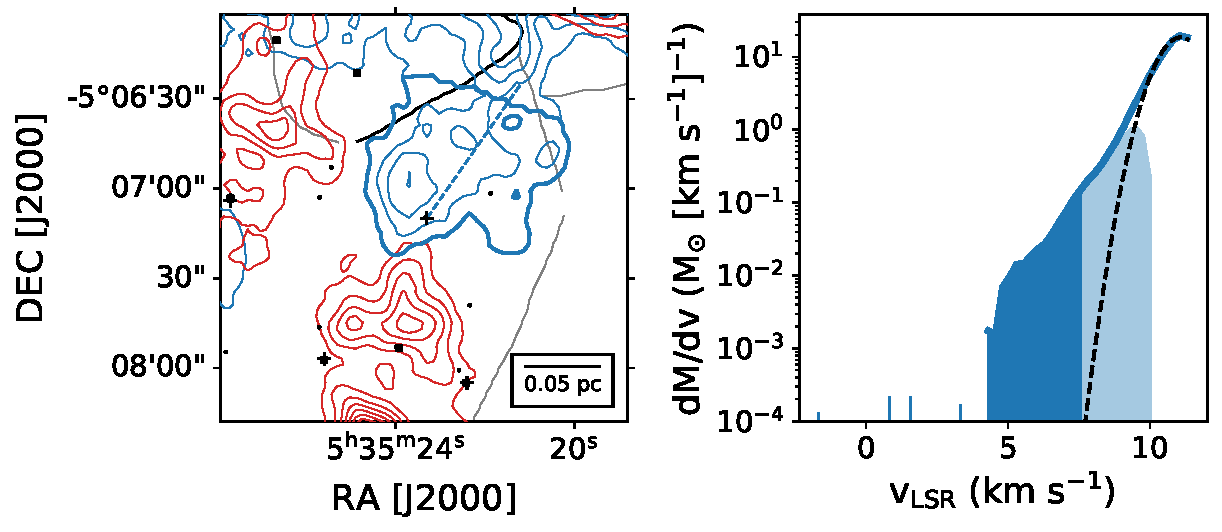
\includegraphics[width=\textwidth]{appendix_figures/davis11.pdf}

    \caption{SMZ 11 outflow. The left panel shows the outflow, position angle, nearby sources, and filaments.
    The velocity range of integration is given by v$_{\rm blue}$/v$_{\rm red}$ in Table~\ref{tab:outflows}
    and the contours go from $5$ to $50\sigma$ in steps of 5$\sigma$, where $\sigma$ is the RMS error in the integrated map. Symbols are the same as Figure~\ref{fig:stamp}.
    The right panel shows the mass spectrum with fit, where $\sigma$ is the RMS error in the integrated map. Symbols are the same as Figure~\ref{fig:dmdv}. The complete figure set (45 images) is available in the online journal.}
    \end{figure*}

